% Document: Bachelor Thesis: Minimal Problem Solver Generator
% Author: Pavel Trutman

\documentclass[msc]{cmpthesis}
\usepackage[czech,english]{babel}
\usepackage[utf8]{inputenc}
\usepackage{indentfirst}
\usepackage{enumitem}
\usepackage{textcomp}
\usepackage{algorithm}
\usepackage{algpseudocode}
\usepackage{listings}
\usepackage{amsmath}
\usepackage{amssymb}
\usepackage{amsthm}
\usepackage{forloop}

\usepackage{subcaption}
\usepackage{pdflscape}
\usepackage{multirow}
\usepackage{dirtree}

% for better verbatim environment
\usepackage{fancyvrb}

% to inlucude pdf pages
\usepackage{pdfpages}

% list of symbols and abbreviations
\usepackage[acronym,nonumberlist,style=long,sort=def]{glossaries}
\setlength{\glsdescwidth}{0.6\linewidth}
\setlength{\glspagelistwidth}{0.4\linewidth}
\renewcommand*{\glsgroupskip}{}
\newcommand{\Acronym}[2]{\newacronym{#1}{#1}{#2}}
\Acronym{cl$(S)$}{Closure of the set $S$}
\Acronym{dom $f$}{Domain of the function $f$}
\Acronym{Dom $f$}{cl(dom $f$)}
\Acronym{int $S$}{Interior of the set $S$}
\newacronym{P}{$\mathcal{P}^n$}{Cone of positive semidefinite $n\times n$ matrices}
\newacronym{S}{$\mathcal{S}^n$}{Space of $n\times n$ real symmetric matrices}
\Acronym{tr$(A)$}{Trace of the matrix $A$}
\newacronym{i-th element of x}{$x^{(i)}$}{$i$-th element of the vector $x$}

\makeglossaries

% algorithmic macros and settings
\newcounter{counter}
\renewcommand{\algorithmicrequire}{\textbf{Input:}}
\renewcommand{\algorithmicensure}{\textbf{Output:}}
\algdef{S}[IF]{IfML}[1]{\algorithmicif\ #1}
\newcommand{\StatexIndent}[1][1]{
  \Statex\forloop{counter}{0}{\value{counter} < #1}{\hskip\algorithmicindent\hskip-0.25em}
}
\renewcommand{\thealgorithm}{\arabic{chapter}.\arabic{algorithm}}
\DeclareCaptionFormat{algorithm}{#1#2#3}
\captionsetup[algorithm]{format=algorithm, labelsep=period}

% listings settings
\makeatletter
\def\lst@numbersymbol{}
\lst@Key{numbersymbol}{}{\def\lst@numbersymbol{#1}}
\lst@Key{numbers}{none}{%
  \let\lst@PlaceNumber\@empty
  \lstKV@SwitchCases{#1}%
  {none&\\%
  left&\def\lst@PlaceNumber{\llap{\normalfont
      \lst@numberstyle{\thelstnumber\lst@numbersymbol}\kern\lst@numbersep}}\\%
  right&\def\lst@PlaceNumber{\rlap{\normalfont
      \kern\linewidth \kern\lst@numbersep
      \lst@numberstyle{\lst@numbersymbol\thelstnumber}}}%
  }{\PackageError{Listings}{Numbers #1 unknown}\@ehc}}
\def\lst@labellis{}
\lst@Key{labellis}{}{\def\lst@label{listing:#1}}
\makeatother
\lstset{basicstyle=\normalfont\ttfamily,
  columns=fixed,
  basewidth=0.5em,
  showstringspaces=false,
  breaklines=true,
  commentstyle=\color{blue},
  keywordstyle=\color{red},
  numbers=left,
  numberstyle=\footnotesize\normalfont,
  numbersymbol=:,
  captionpos=t,
  frame=top,
  frame=bottom,
  xleftmargin=25pt,
  framexleftmargin=25pt,
}
\DeclareCaptionFormat{listing}{\rule{\dimexpr\textwidth\relax}{1pt}\vskip-3pt\hspace{-10pt}#1#2#3}
\captionsetup[lstlisting]{format=listing, singlelinecheck=false, labelsep=period}
\renewcommand\lstlistlistingname{List of Listings}

\startThesisInfo
\title{Semidefinite Programming for Geometric Problems in Computer Vision}
\author{Pavel Trutman}
\CMPAdvisor{Ing. Tom\'a\v s Pajdla, PhD.}
\CMPReportNo{}
\CMPAcknowledgement{\centering }

\CMPEmail{pavel.trutman@fel.cvut.cz}
\CMPDocumentURL{http://cmp.felk.cvut.cz/~trutmpav/master-thesis/thesis/thesis.pdf}
\stopThesisInfo

% ============================== your definitions (abbreviations etc.)
\newcommand{\eqB}{\begin{eqnarray}}
\newcommand{\eqE}{\end{eqnarray}}
\newcommand{\bmB}{\begin{bmatrix}}
\newcommand{\bmE}{\end{bmatrix}}
\newcommand{\ind}[1]{\ensuremath{^{(#1)}}}
\newcommand{\labeldef}[1]{\label{definition:#1}}
\newcommand{\refdef}[1]{Definition~\ref{definition:#1}}
\newcommand{\labelcol}[1]{\label{corollary:#1}}
\newcommand{\refcol}[1]{Corollary~\ref{corollary:#1}}
\newcommand{\labelthe}[1]{\label{theorem:#1}}
\newcommand{\refthe}[1]{Theorem~\ref{theorem:#1}}
\newcommand{\labelex}[1]{\label{example:#1}}
\newcommand{\refex}[1]{Example~\ref{example:#1}}
\newcommand{\labeleq}[1]{\label{equation:#1}}
\newcommand{\refeqb}[1]{(\ref{equation:#1})}
\newcommand{\labelalg}[1]{\label{algorithm:#1}}
\newcommand{\refalg}[1]{Algorithm~\ref{algorithm:#1}}
\newcommand{\labelalgline}[1]{\label{algorithm:line:#1}}
\newcommand{\refalgline}[1]{\ref{algorithm:line:#1}}
\newcommand{\labelfig}[1]{\label{figure:#1}}
\newcommand{\reffig}[1]{Figure~\ref{figure:#1}}
\newcommand{\labelsec}[1]{\label{section:#1}}
\newcommand{\refsec}[1]{Section~\ref{section:#1}}
\newcommand{\reflis}[1]{Listing~\ref{listing:#1}}
\newtheoremstyle{definitionStyle}
  {}
  {}
  {}
  {}
  {\bfseries}
  {.}
  { }
  {\thmname{#1}\thmnumber{ #2}\thmnote{ (#3)}}
\theoremstyle{definitionStyle}
\newtheorem{definition}{Definition}[chapter]
\newtheorem{theorem}{Theorem}[chapter]
\newtheorem{example}{Example}[chapter]
\newtheorem{corollary}{Corollary}[chapter]
\newcommand{\R}{\mathbb{R}}
\newcommand{\Sym}{\mathcal{S}}
\newcommand{\PSDCone}{\mathcal{P}}
\DeclareMathOperator{\rank}{rank}
\DeclareMathOperator{\dom}{dom}
\DeclareMathOperator{\Dom}{Dom}
\DeclareMathOperator{\cl}{cl}
\DeclareMathOperator{\inter}{int}
\DeclareMathOperator{\tr}{tr}

\setitemize{noitemsep,topsep=0.2cm,parsep=0.2cm,partopsep=0pt,leftmargin=1cm}
\setenumerate{noitemsep,topsep=0.2cm,parsep=0.2cm,partopsep=0pt,leftmargin=1cm}

% =========================================================== settings
\graphicspath{{images/}}

% ========================================================== text body
\begin{document}

\cleardoublepage\def\thepage{\roman{page}}\setcounter{page}{3}

% thesis assignment as required by FEE, CTU
%
\includepdf[pages={1}]{pdfs/assignment-ENG.pdf}
%\includepdf[pages={1}]{pdfs/assignment-CZE.pdf}

\mbox{}\vfill

{\let\clearpage\relax\par \chapter*{Acknowledgements}}
I would like to express my thanks to my advisor Tom\'a\v s Pajdla for his guidance and valuable advices, which enabled me to finish this thesis.
I would also like to thank Didier Herion for introducing me into semidefinite programming and polynomial optimization techniques and for his useful discussion and comments to my work.
Special thanks go to my family for all their support.

\clearpage
\mbox{}\vfill

{\let\clearpage\relax\par \chapter*{Author's declaration}}
I declare that the presented work was developed independently and that I have listed all sources of information used within it in accordance with the methodical instructions for observing the ethical principles in the preparation of university theses.

%{\let\clearpage\relax\par \chapter*{Prohl\'a\v sen\'i autora pr\'ace}}
%Prohla\v suji, \v ze jsem p\v redlo\v zenou pr\' aci vypracoval samostatn\v e a \v ze jsem uvedl ve\v sker\'e pou\v zit\'e informa\v cn\'i zdroje v souladu s Metodick\'ym pokynem o dodr\v zov\'an\'i etick\'ych princip\r u p\v ri p\v r\'iprav\v e vysoko\v skolsk\'ych z\'av\v ere\v cn\'ych prac\'i.

\vskip3cm
\begin{tabular}{lp{1cm}c}
  Prague, date \makebox[4cm]{\dotfill} &  & \makebox[5cm]{\dotfill}\\
  & & Signature
\end{tabular}

\clearpage
\chapter*{Abstract}
Many problems in computer vision lead to polynomial systems solving.
The state of the art algebraic methods for polynomial systems solving are able to efficiently solve the systems over complex numbers, but the non-real solutions are then discarded, as they are not solutions of the original geometric problems.
On this purpose, we review and implement the moment method for polynomial systems solving, which solves the problems over real numbers directly.
We show that the moment method is applicable to the minimal problems from computer vision geometry.
For that, we give description of the calibrated camera pose problem and of the calibrated camera pose with unknown focal length problem.
We compare our implementation of the moment with the state of the art methods on these two selected minimal problems on real 3D scene.

Moreover, we review and implement a method for solving polynomial optimization problems, which can extend the moment method with inequality constraints.
This method uses Lasserre's hierarchies to find the optimal values of the original optimization problems.
We compare the performance of our implementation with the state of the art methods on synthetically generated polynomial optimization problems.

Since the semidefinite programs solving is a key element in the moment method and the polynomial optimization methods, we review and implement an interior-point algorithm for semidefinite programs solving.
We compare the performance of our implementation with the state of the art methods on synthetically generated semidefinite programs.

\paragraph{Keywords:}
computer vision, polynomial systems solving, polynomial optimization, semidefinite programming, minimal problems

\begin{otherlanguage}{czech}
\chapter*{Abstrakt}
Mnoho problémů v počítačovém vidění vede na řešení systémů polynomiálních rovnic.
Současné metody na řešení systémů polynomiálních rovnic jsou schopny řešit tyto systémy v oboru komplexních čísel, ale následně jsou nereálná řešení vyřazena, protože ta nejsou řešeními původních geometrických problémů.
Z tohoto důvodu prozkoumáme a implementujeme metodu momentů pro řešení systémů polynomiálních rovnic, která řeší tyto problémy přímo v oboru reálných čísel.
Ukážeme, že metoda momentů je použitelná na minimální problémy z geometrie počítačového vidění.
Proto popíšeme problém nalezení polohy kalibrované kamery a problém nalezení polohy kalibrované kamery s neznámou ohniskovou vzdáleností.
Na těchto dvou vybraných minimálních problémech a reálné 3D scéně porovnáme naší implementaci metody momentů se sou\-čas\-ný\-mi metodami.

Dále prozkoumáme a implementujeme metodu na řešení polynomiálně optimalizačních problémů, která může rozšířit metodu momentů o omezení s nerovnostmi.
Tato metoda využívá Lasserrových hierarchií k nalezení optimálních hodnot původních optimalizačních problémů.
Na synteticky generovaných polynomiálně optimalizačních prob\-lé\-mech porovnáme výkon naší implementace se současnými metodami.

Protože řešení semidefinitních programů je klíčovým elementem metody momentů a metod polynomiální optimalizace, prozkoumáme a implementujeme algoritmus vnitřních bodů na řešení semidefinitních programů.
Na synteticky generovaných semidefinitních problémech porovnáme výkon naší implementace se současnými metodami.

\paragraph{Klíčová slova:}
počítačové vidění, řešení polynomiálních systémů, polynomiální optimalizace, semidefinitní programování, minimální problémy
\end{otherlanguage}

\clearpage
\cleardoublepage\def\thepage{\arabic{page}}\setcounter{page}{1}
\tableofcontents\pagestyle{headings}
\listoffigures
\listofalgorithms
\lstlistoflistings

\glsaddall
\printglossary[type=acronym,title=List of Symbols and Abbreviations]

\chapter{Introduction}
In geometry of computer vision, many problems are formulated as systems of polynomial equations.
The state of the art methods are based on polynomial algebra, i.e.\ on Gr\"obner bases and multiplication matrices computation.
Contrary to this approach, this work applies non-linear optimization techniques to solve the polynomial systems, which is a novel idea in the field of geometry of computer vision.
Moreover, the application of the optimization techniques allows us to enrich the polynomial systems with polynomial inequalities or to solve polynomial optimization problems, i.e.\ optimizing a polynomial function with given polynomial constraints.

\section{Motivation}
Object recognition and localization, reconstruction of 3D scenes, self-driving cars, film production, augmented reality and robotics are only few of many applications of geometry of computer vision.
Thus, one would like to solve geometric problems efficiently, since these problems often have to be solved in real-time applications.
Typical geometric problems from computer vision are the minimal problems, which arise when estimating geometric models of scenes from given images.
To be able to solve these problems computationally, they are often represented by systems of algebraic equations.
Hence, one of the issues of computer vision is, how to solve systems of polynomial equations efficiently, which is the scope of this work.

The polynomial systems obtained from the geometric problems are often not trivial, but usually consist of many polynomial equations of high degree in several unknowns.
From that reason, general algorithms for polynomial systems solving are not efficient for them, and therefore special solvers have been developed for different problems to solve these problems efficiently and robustly.
Previously, these solvers were handcrafted, which is quite time demanding process that has to be done for each problem from scratch.
Then, the process was automated by automatic generators \cite{autogen, larsson}, which automatically generate efficient solver for a given type of the polynomial system.
These solvers obtain the Gr\"obner basis of the system and then construct the multiplication matrix, from which solutions are extracted by eigenvectors computation.
The side effect of this approach is that some non-real solutions often appear amongst real solutions, which are not solutions to the original geometric problem.
Since the computation of the non-real solutions takes time, a method which would find real solutions only may be faster than the contemporary approach.

Some of the arisen systems may be overconstrained.
Such systems have a solution when solved on precise data using precise arithmetic, but they have no solution when solved on real noisy data.
However, these systems may be transformed into optimization problem by relaxing some of the constrains and by minimizing the error of these constraints.
Therefore, an efficient polynomial optimization method may prove useful for overconstrained systems.

\section{Contributions}
To solve polynomial systems over real numbers only, we apply the moment method introduced by J. B. Lasserre et al.
This method uses hierarchies of semidefinite programs to find a Gr\"obner basis of real radical ideal constructed from the ideal generated by the given polynomials.
Then, a multiplication matrix is constructed and solutions are obtained from it.
In this case, the multiplication matrix should have smaller size than a multiplication matrix obtained from the automatic generator, which can save some computation time.
We implement this method in Python and MATLAB and examine its properties on several minimal problems from geometry of computer vision on real 3D scenes.
We show that this method is applicable on problems from computer vision.

The second contribution of this work is, that we describe and review a method for polynomial optimization problems.
This method solves hierarchies of semidefinite programs to find the optimal value.
An application of this method can, for example, be a solver of overconstrained polynomial systems.
We implement our own implementation of this method in Python and compare it to the state of the art methods on synthetic polynomial optimization problems.

Since semidefinite programs solving is a key element in both previously mentioned methods, we review and describe an interior-point method for semidefinite programs solving.
To be able to use this method in implementations of the moment method and the polynomial optimization method, we implement this interior-point method in Python.
To verify our implementation we compare it to the state of the art semidefinite solvers on synthetic semidefinite programs.

\section{Thesis structure}
In this work, we first review an interior-point method for semidefinite programs solving.
To do so, general properties of self-concordant functions and barriers need to be introduced, since they are key elements in convex optimization.
Then, a specialized barrier function for semidefinite programming will be described.
%The knowledge of semidefinite programming is important for us, since it plays crucial role in polynomial optimization techniques described later in the text.
We describe our implementation of the semidefinite programs solver and compare it to the state of the art methods.

Secondly, we focus on polynomial optimization.
After an introduction to polynomial algebra and moment matrices, we describe and implement a method, which solves polynomial optimization problems by relaxations of semidefinite programs.
Then, we review the moment method and describe its implementation in Python.
%The moment method allows us to solve systems of polynomial equations over real numbers.

To compare the implementation of the moment method to the state of the art methods, we introduce two minimal problems from computer vision on which we perform the experiments.
The minimal problems are the estimation (i) of the calibrated camera pose and (ii) of the calibrated camera pose with unknown focal length.
We show that our implementation of the moment method is applicable to these selected geometric problems from computer vision.


\chapter{Semidefinite programming}
The goal of the semidefinite programming (SDP) is to optimize a linear function on a given set, which is an intersection of a cone of positive semidefinite matrices with an affine space.
This set is called a spectrahedron and it is a convex set.
Since in SDP we are optimizing a convex function on a convex set, SDP is a special case of convex optimization.

Since SDP can be solved efficiently in polynomial time using interior-point method, it has many applications in practise.
For example, any linear program (LP) and quadratically constrained quadratic program (QCQP) can be written as a semidefinite program.
However, this may be not the best idea to do as more efficient algorithms exist for solving LPs and QCQPs.
On the other hand, there exist many useful applications of SDP, e.g.\ many NP-complete problems in combinatorial optimization can be approximated by semidefinite programs. 
One of the combinatorial problem worth mentioning is the MAX CUT problem (one of the Karp's original NP-complete problems \cite{karp1972}), for which M. Goemans and D. P. Williamson created the first approximation algorithm based on SDP \cite{max-cut}.
Also in control theory, there are many problems based on linear matrix inequalities, which are solvable by SDP.
Special application of SDP comes from polynomial optimization since global solution of polynomial optimization problems can be found by hierarchies of semidefinite programs.
We will focus in details on this application in \refsec{poly}.

\section{Preliminaries on semidefinite programs}
We introduce here some notation and preliminaries about symmetric matrices and semidefinite programs.
We will introduce further notation and preliminaries later on in the text when needed.

At the beginning, let us denote the inner product for two vectors $x$, $y \in\R^n$
\begin{eqnarray}
  \langle x, y\rangle &=& \sum_{i=1}^n x\ind{i}y\ind{i}
\end{eqnarray}
and the Frobenius inner product for two matrices $X$, $Y\in\R^{n\times m}$.
\begin{eqnarray}
  \langle X, Y\rangle &=& \sum_{i=1}^n \sum_{j=1}^m X\ind{i,j}Y\ind{i,j}
\end{eqnarray}

\subsection{Symmetric matrices}
Let $\Sym^n$ denotes the space of $n\times n$ real symmetric matrices.

For a matrix $M\in\Sym^n$, the notation $M \succeq 0$ means that $M$ is positive semidefinite.
$M \succeq 0$ if and only if any of the following equivalent properties holds.
\begin{enumerate}
  \item $x^\top Mx \geq 0$ for all $x \in \R^n$.
  \item All eigenvalues of $M$ are nonnegative.
\end{enumerate}
The set of all positive semidefinite matrices is a cone.
We will denote it as $\PSDCone^n$ and it is called a cone of positive semidefinite matrices.

For a matrix $M\in\Sym^n$, the notation $M \succ 0$ means that $M$ is positive definite.
$M \succ 0$ if and only if any of the following equivalent properties holds.
\begin{enumerate}
  \item $M \succeq 0$ and $\rank M = n$.
  \item $x^\top Mx > 0$ for all $x \in \R^n$.
  \item All eigenvalues of $M$ are positive.
\end{enumerate}

\subsection{Semidefinite programs}
The standard (primal) form of a semidefinite program in variable $X\in\Sym^n$ is defined as follows:
\begin{eqnarray}
  \begin{array}{rclrrclcll}
    p^* &=& \displaystyle \sup_{X\in\Sym^n} & \multicolumn{3}{l}{\langle C,X\rangle} \\
    && \text{s.t.} & \langle A_i, X\rangle &=& b\ind i & (i = 1,\ldots,m)\\
    &&& X &\succeq& 0
  \end{array}
\end{eqnarray}
where $C$, $A_1$, \ldots, $A_m \in \Sym^n$ and $b\in\R^m$ are given.

The dual form of the primal form is the following program in variable $y\in\R^m$.
\begin{eqnarray}
  \begin{array}{rclrrclcll}
    d^* &=& \displaystyle \inf_{y\in\R^m} & \multicolumn{3}{l}{b^\top y} \\
    && \text{s.t.} & \displaystyle \sum_{i=1}^m A_iy\ind i - C &\succeq& 0
  \end{array}\labeleq{SDP:prelim:dual}
\end{eqnarray}
The constraint 
\begin{eqnarray}
  F(y) &=& \sum_{i=1}^m A_iy\ind i - C\ \succeq\ 0
\end{eqnarray}
of the problem \refeqb{SDP:prelim:dual} is called a linear matrix inequality (LMI) in the variable $y$.
The feasible region defined by LMI is called a spectrahedron.
It can be shown, that this constraint is convex since if $F(x) \succeq 0$ and $F(y) \succeq 0$, then $\forall \alpha: 0\leq  \alpha \leq 1$ holds
\begin{eqnarray}
  F\big(\alpha x + (1-\alpha)y\big) &=& \alpha F(x) + (1-\alpha)F(y)\ \succeq \ 0.
\end{eqnarray}
The objective function of the problem \refeqb{SDP:prelim:dual} is linear, and therefore convex too.
Because the semidefinite program \refeqb{SDP:prelim:dual} has convex objective function and convex constraint, it is a convex optimization problem and can be solved by standard convex optimization methods.
To get a general picture, how a simple semidefinite problem may look like, see \reffig{SDP:prelim:problem}.

\begin{figure}[ht]
  \centering
  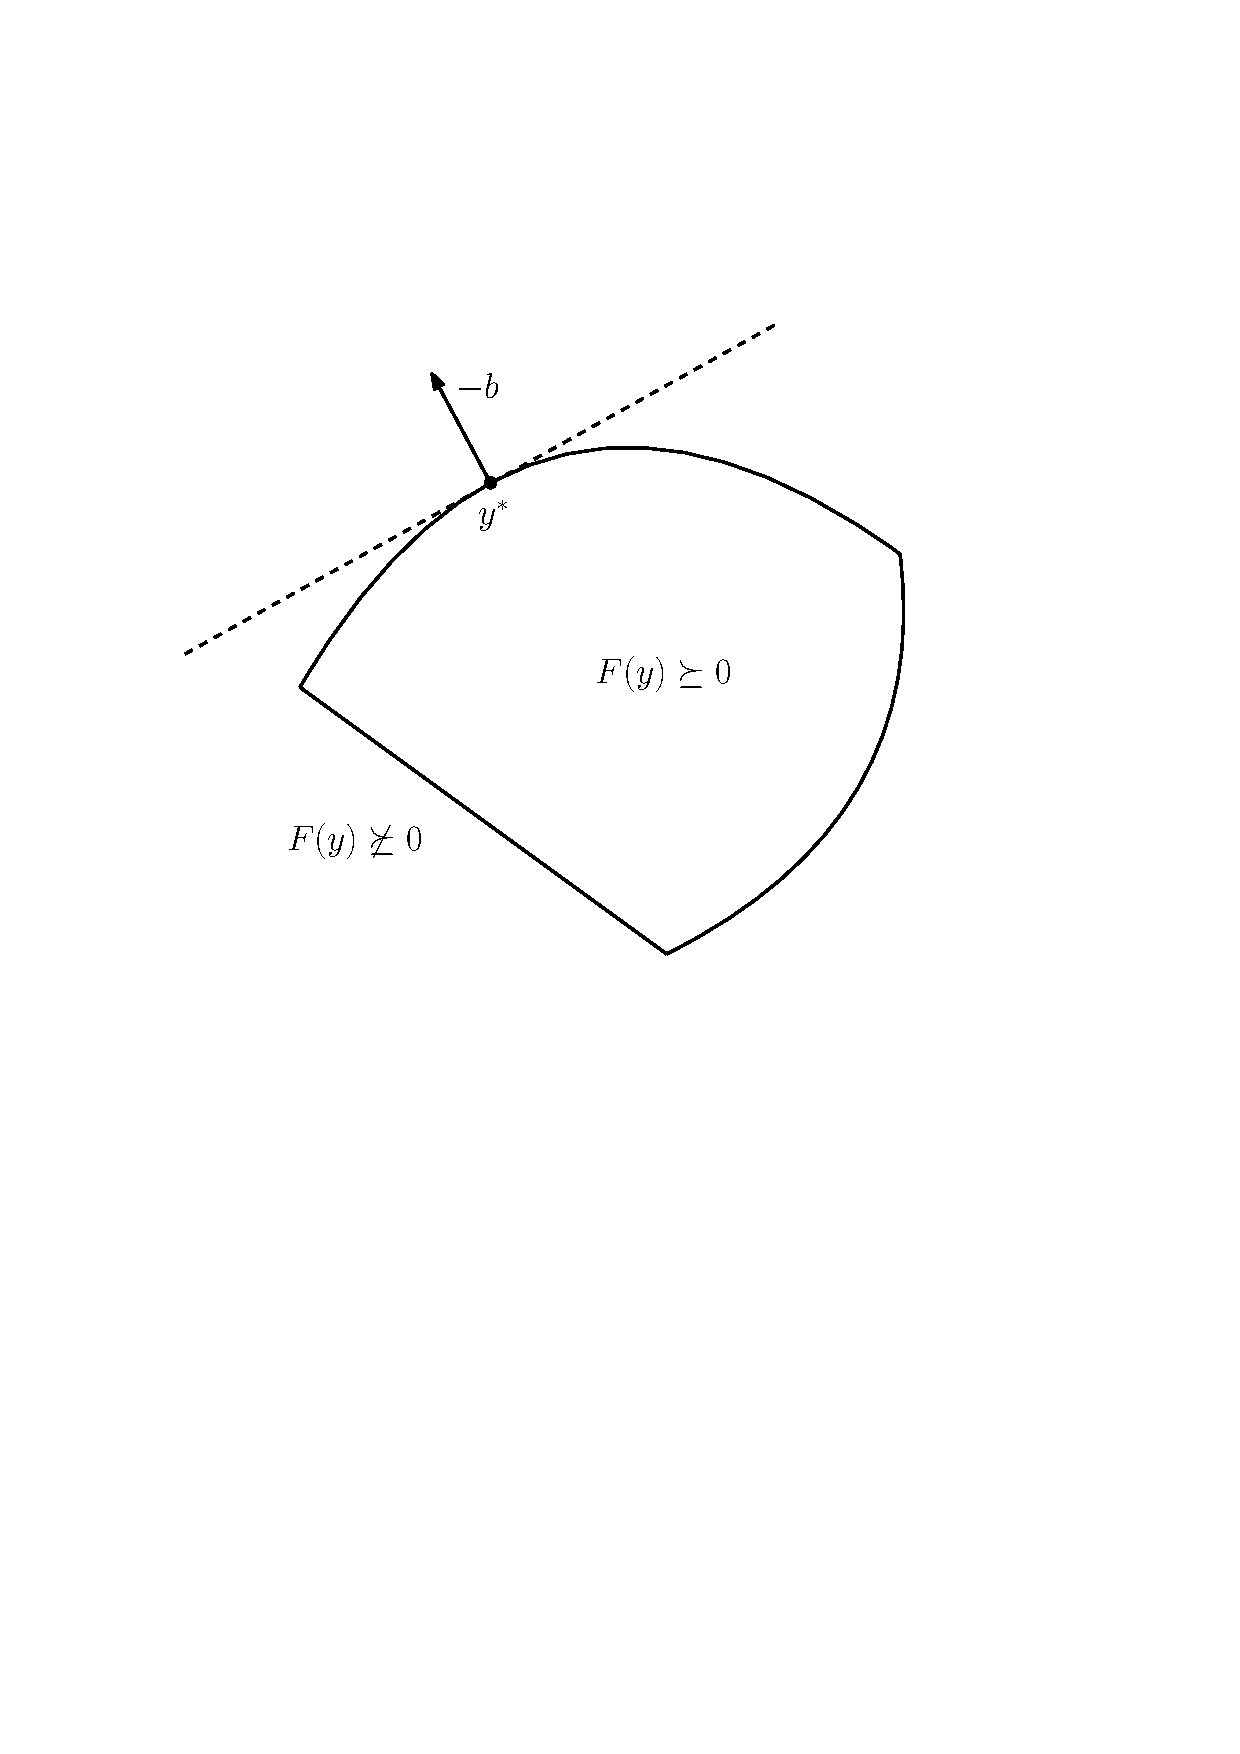
\includegraphics[width=0.5\textwidth]{drawings/SDP_problem.pdf}
  \caption{Example of a simple semidefinite problem for $y\in\R^2$. Boundary of the feasible set $\big\{y\ |\ F(y)\succeq 0\big\}$ is shown as a black curve. The minimal value of the objective function $b^\top y$ is attained at $y^*$.}
  \labelfig{SDP:prelim:problem}
\end{figure}

The optimal solution $y^*$ of any semidefinite program lies on the boundary of the feasible set, supposing the problem is feasible and the solution exists.
The boundary of the feasible set is not smooth in general, but it is piecewise smooth as each piece is an algebraic surface.

\begin{example}[Linear programming]
  Semidefinite programming can be seen as an extension to the linear programming since the componentwise inequalities between vectors in linear programming can be replaced by LMI.
  Consider a linear program in a standard form
  \begin{eqnarray}
    \begin{array}{rclrrclcll}
      y^* &=& \displaystyle \arg\min_{y\in\R^m} & \multicolumn{3}{l}{b^\top y} \\
      && \text{s.t.} & \displaystyle Ay - c &\geq& 0
    \end{array}
  \end{eqnarray}
  with $b\in\R^m$, $c\in\R^n$ and $A = \bmB a_1 & \ldots & a_m \bmE \in\R^{n\times m}$.
  This program can be transformed into the semidefinite program \refeqb{SDP:prelim:dual} by assigning
  \begin{eqnarray}
    C &=& \diag(c),\\
    A_i &=& \diag(a_i).
  \end{eqnarray}
\end{example}

\section{State of the art review}
An early paper by R. Bellman and K. Fan about theoretical properties of semidefinite programs \cite{Bellman-Fan} was issued in 1963.
Later on, many researchers worked on the problem of minimizing the maximal eigenvalue of a symmetric matrix, which can be done by solving a semidefinite program.
Selecting a few from many: J. Cullum, W. Donath, P. Wolfe \cite{Cullum-Donath-Wolfe}, M. Overton \cite{Overton} and G. Pataki \cite{Pataki}.
In 1984, the interior-point methods for LPs solving were introduced by N. Karmarkar \cite{Karmarkar1984}.
It was the first reasonably efficient algorithm that solves LPs in polynomial time with excellent behavior in practise.
The interior-point algorithms were then extended to be able to solve convex quadratic programs.

In 1988, Y. Nesterov and A. Nemirovski \cite{Nesterov-Nemirovski} did an important breakthrough.
They showed that interior-point methods developed for LPs solving can be generalized to all convex optimization problems.
All that is required, is the knowledge of a self-concordant barrier function for the feasible set of the problem.
Y. Nesterov and A. Nemirovski have shown that a self-concordant barrier function exists for every convex set.
However their proposed universal self-concordant barrier function and its first and second derivatives are not easily computable.
Fortunately, for SDP, which is an important class of convex optimization programs, computable self-concordant barrier functions are known, and therefore the interior-point methods can be used.

Nowadays, there are many libraries and toolboxes that one can use for solving semidefinite programs.
They differ to each other in used methods and their implementations.
Before starting solving a problem, one should know the details of the problem to solve and choose the library accordingly to it as not every method and its implementation is suitable for the given problem.

Most methods are based on interior-point methods, which are efficient and robust for general semidefinite programs.
The main disadvantage of these methods is that they need to store and factorize usually large Hessian matrix.
Most modern implementations of the interior-point methods do not need the knowledge of an interior feasible point in advance.
SeDuMi \cite{sedumi} casts the standard semidefinite program into the homogeneous self-dual form, which has a trivial feasible point.
SDPA \cite{sdpa} uses an infeasible interior-point method, which can initialized by an infeasible point.
Some of the libraries (e.g.\ MOSEK \cite{mosek}) have started out as LPs solvers and were extended for QCQPs solving and convex optimization later on.

Another type of methods used in SDP are the first-order methods. 
They avoid storing and factorizing Hessian matrices, and therefore they are able to solve much larger problems than interior-point methods, but at some cost in accuracy.
This method is implemented, for instance, in the SCS solver \cite{scs}.

\section{Nesterov's approach}
In this section, we will follow Chapter 4 of \cite{Nesterov-2004} by Y. Nesterov, which is devoted to the convex optimization problems.
This chapter describes the state of the art interior-point methods for solving convex optimization problems.
We will extract from it the only minimum, just to be able to introduce an algorithm for semidefinite programs solving.
We will present some basic definitions and theorems, but we will not prove them.
For the proofs and more details look into \cite{Nesterov-2004}.

\subsection{Self-concordant functions}
\begin{definition}[Self-concordant function in $\R$]
  A closed convex function $f: \R \mapsto \R$ is self-concordant if there exist a constant $M_f \geq 0$ such that the inequality
  \begin{eqnarray}
    |f'''(x)| &\leq& M_f f''(x)^{3/2}
  \end{eqnarray}
  holds for all $x\in\dom f$.
\end{definition}

For better understanding of self-concordant functions, we provide several examples.

\begin{example}~
  \begin{enumerate}
    \item Linear and convex quadratic functions.
      \begin{eqnarray}
        f'''(x) &=& 0\ \text{ for all } x
      \end{eqnarray}
      Linear and convex quadratic functions are self-concordant with constant $M_f = 0$.
    \item Negative logarithms.
      \begin{eqnarray}
        f(x) &=& -\ln(x)\ \text{ for } x>0\\
        f'(x) &=& -\frac{1}{x}\\
        f''(x) &=& \frac{1}{x^2}\\
        f'''(x) &=& -\frac{2}{x^3}\\
        \frac{|f'''(x)|}{f''(x)^{3/2}} &=& 2
      \end{eqnarray}
      Negative logarithms are self-concordant functions with constant $M_f = 2$.

    \item Exponential functions.
      \begin{eqnarray}
        f(x) &=& e^x\\
        f''(x) \ =\ f'''(x) &=& e^x\\
        \frac{|f'''(x)|}{f''(x)^{3/2}} &=& e^{-x/2} \rightarrow+\infty \ \text{ as } x\rightarrow-\infty
      \end{eqnarray}
      Exponential functions are not self-concordant functions.
  \end{enumerate}
\end{example}

\begin{definition}[Self-concordant function in $\R^n$]
  A closed convex function $f: \R^n \mapsto \R$ is self-concordant if function
  \begin{eqnarray}
    g(t) &=& f(x + tv)
  \end{eqnarray}
  is self-concordant for all $x\in\dom f$ and all $v\in\R^n$.
\end{definition}

Now, let us focus on the main properties of self-concordant functions.

\begin{theorem}
  Let functions $f_i$ be self-concordant with constants $M_i$  and let $\alpha_i > 0$, $i = 1,2$. Then the function
 \begin{eqnarray}
   f(x) &=& \alpha_1f_1(x) + \alpha_2f_2(x)
 \end{eqnarray}
 is self-concordant with constant
 \begin{eqnarray}
   M_f &=& \max \bigg\{\frac{1}{\sqrt{\alpha_1}}M_1, \frac{1}{\sqrt{\alpha_2}}M_2\bigg\}
 \end{eqnarray}
 and
 \begin{eqnarray}
   \dom f &=& \dom f_1 \cap \dom f_2.
 \end{eqnarray}
\end{theorem}

\begin{corollary}\labelcol{SDP:scf:scaling}
  Let function $f$ be self-concordant with some constant $M_f$ and $\alpha > 0$. Then the function $\phi(x) = \alpha f(x)$ is also self-concordant with the constant $M_\phi = \frac{1}{\sqrt{\alpha}}M_f$.
\end{corollary}

We call function $f(x)$ as the standard self-concordant function if $f(x)$ is some self-concordant function with the constant $M_f = 2$. Using \refcol{SDP:scf:scaling}, we can see that any self-concordant function can be transformed into the standard self-concordant function by scaling.

\begin{theorem}\labelthe{SDP:scf:hessian}
  Let function $f$ be self-concordant. If $\dom f$ contains no straight line, then the Hessian $f''(x)$ is nondegenerate at any $x$ from $\dom f$.
\end{theorem}

For some self-concordant function $f(x)$, for which we assume, that $\dom f$ contains no straight line (which implies that all $f''(x)$ are nondegenerate, see \refthe{SDP:scf:hessian}), we denote two local norms as
\begin{eqnarray}
  \| u \|_x &=& \sqrt{u^\top f''(x) u}\\
  \| u \|_x^* &=& \sqrt{u^\top f''(x)^{-1} u}.
\end{eqnarray}

Consider following minimization problem
\begin{eqnarray}
  x^* &=& \arg\min_{x\in\dom f} f(x)\labeleq{SDP:scf:minProblem}
\end{eqnarray}
as the minimization of the self-concordant function $f(x)$.
\refalg{SDP:scf} is describing the iterative process of solving optimization problem \refeqb{SDP:scf:minProblem}.
The algorithm is divided into two stages by the value of $\|f'(x_k)\|_{x_k}^*$.
The splitting parameter $\beta$ guarantees quadratic convergence rate for the second part of the algorithm. The parameter $\beta$ is chosen from interval $(0, \bar{\lambda})$, where
\begin{eqnarray}
  \bar{\lambda} &=& \frac{3 - \sqrt{5}}{2},
\end{eqnarray}
which is a root of the equation
\begin{eqnarray}
  \frac{\lambda}{(1-\lambda)^2} &=& 1.
\end{eqnarray}

\begin{algorithm}[ht]
  \begin{algorithmic}[1]
    \Require
      \Statex $f$ a self-concordant function to minimize
      \Statex $x_0 \in \dom f$ a starting point
      \Statex $\beta \in (0,\bar{\lambda})$ a parameter of size of the region of quadratic convergence
      \Statex $\varepsilon$ a precision
    \Ensure
      \Statex $x^*$ an optimal solution to the minimization problem \refeqb{SDP:scf:minProblem}
      \Statex

    \State $k \gets 0$
    \While{$\|f'(x_k)\|_{x_k}^* \geq \beta$} \labelalgline{SDP:scf:w1b}
      \State $x_{k+1} \gets x_k - \frac{1}{1+\|f'(x_k)\|_{x_k}^*}f''(x_k)^{-1}f'(x_k)$
      \State $k \gets k + 1$
    \EndWhile \labelalgline{SDP:scf:w1e}
    \While{$\|f'(x_k)\|_{x_k}^* > \varepsilon$} \labelalgline{SDP:scf:w2b}
      \State $x_{k+1} \gets x_k - f''(x_k)^{-1}f'(x_k)$
      \State $k \gets k + 1$
    \EndWhile \labelalgline{SDP:scf:w2e}
    \State \Return $x^* \gets x_k$

  \end{algorithmic}
  \caption{Newton method for minimization of the self-concordant functions.}
  \labelalg{SDP:scf}
\end{algorithm}


The first while loop (lines \refalgline{SDP:scf:w1b} -- \refalgline{SDP:scf:w1e}) represents damped Newton method, where at each iteration we have
\begin{eqnarray}
  f(x_k) - f(x_{k+1}) &\geq& \beta - \ln(1+\beta) \text{ for } k \geq 0,
\end{eqnarray}
where
\begin{eqnarray}
  \beta - \ln(1+\beta) &>& 0 \text{ for } \beta > 0,
\end{eqnarray}
and therefore the global convergence of the algorithm is ensured.
It can be shown that the local convergence rate of the damped Newton method is also quadratic, but the presented switching strategy is preferred as it gives better complexity bounds.

The second while loop of the algorithm (lines \refalgline{SDP:scf:w2b} -- \refalgline{SDP:scf:w2e}) is the standard Newton method with quadratic convergence rate.

The algorithm terminates when the required precision $\varepsilon$ is reached.


\subsection{Self-concordant barriers}
To be able to introduce self-concordant barriers, let us denote $\Dom f = \cl(\dom f)$.

\begin{definition}[Self-concordant barrier]\labeldef{SDP:scb:scb}
  Let $F(x)$ be a standard self-concordant function. We call it a $\nu$-self-concordant barrier for set $\Dom F$, if
  \begin{eqnarray}
    \sup_{u\in\R^n} \big(2u^\top F'(x) - u^\top F''(x) u\big) &\leq& \nu \labeleq{SDP:scb:def}
  \end{eqnarray}
  for all $x\in\dom F$. The value $\nu$ is called the parameter of the barrier.
\end{definition}

The inequality \refeqb{SDP:scb:def} can be rewritten into the following equivalent matrix notation:
\begin{eqnarray}
  F''(x) &\succeq& \frac{1}{\nu}F'(x)F'(x)^\top.\labeleq{SDP:scb:def1}
\end{eqnarray}

In \refdef{SDP:scb:scb}, the hessian $F''(x)$ is not required to be nondegenerate. However, in case that $F''(x)$ is nondegenerate, the inequality \refeqb{SDP:scb:def} is equivalent to
\begin{eqnarray}
  F'^\top(x)F''(x)^{-1}F'(x) &\leq& \nu.\labeleq{SDP:scb:def2}
\end{eqnarray}

Let us explore, which basic functions are self-concordant barriers.

\begin{example}~
  \begin{enumerate}
    \item Linear functions.
      \begin{eqnarray}
        F(x) &=& \alpha + a^\top x,\ \dom F = \R^n\\
        F''(x) &=& 0
      \end{eqnarray}
      From \refeqb{SDP:scb:def1} and for $a \neq 0$ follows, that linear functions are not self-concordant barriers.

    \item Convex quadratic functions.\\
      For $A = A^\top \succ 0$:
      \begin{eqnarray}
        F(x) &=& \alpha + a^\top x + \frac{1}{2} x^\top Ax,\ \dom F = \R^n\\
        F'(x) &=& a + Ax\\
        F''(x) &=& A
      \end{eqnarray}
      After substitution into \refeqb{SDP:scb:def2} we obtain
      \begin{eqnarray}
        (a + Ax)^\top A^{-1}(a + Ax) &=& a^\top A^{-1}a + 2a^\top x + x^\top Ax,
      \end{eqnarray}
      which is unbounded from above on $\R^n$. Therefore, quadratic functions are not self-concordant barriers.
      

    \item Logarithmic barrier for a ray.
      \begin{eqnarray}
        F(x) &=& -\ln x,\ \dom F = \big\{x\in\R\ |\ x > 0\big\}\\
        F'(x) &=& -\frac{1}{x}\\
        F''(x) &=& \frac{1}{x^2}
      \end{eqnarray}
      From \refeqb{SDP:scb:def2}, when $F'(x)$ and $F''(x)$ are both scalars, we get
      \begin{eqnarray}
        \frac{F'(x)^2}{F''(x)} &=& \frac{x^2}{x^2}\ =\ 1.
      \end{eqnarray}
      Therefore, the logarithmic barrier for a ray is a self-concordant barrier with parameter $\nu = 1$ on domain $\big\{x\in\R\ |\ x > 0\big\}$.
  \end{enumerate}
\end{example}

Now, let us focus on the main properties of self-concordant barriers.

\begin{theorem}\labelthe{SDP:scb:penaltyFunction}
  Let $F(x)$ be a self-concordant barrier. Then the function $c^\top x + F(x)$ is a self-concordant function on $\dom F$.
\end{theorem}

\begin{theorem}
  Let $F_i$ be $\nu_i$-self-concordant barriers, $i = 1,2$. Then the function
  \begin{eqnarray}
    F(x) &=& F_1(x) + F_2(x)
  \end{eqnarray}
  is a self-concordant barrier for convex set
  \begin{eqnarray}
    \Dom F &=& \Dom F_1 \cap \Dom F_2
  \end{eqnarray}
  with the parameter
  \begin{eqnarray}
    \nu &=& \nu_1 + \nu_2.
  \end{eqnarray}
\end{theorem}

\begin{theorem}\labelthe{SDP:scb:distance}
  Let $F(x)$ be a $\nu$-self-concordant barrier. Then for any $x\in\Dom F$ and $y\in\Dom F$ such that
  \begin{eqnarray}
    (y-x)^\top F'(x) &\geq& 0,
  \end{eqnarray}
  we have
  \begin{eqnarray}
    \|y-x\|_x &\leq& \nu + 2\sqrt{\nu}.
  \end{eqnarray}
\end{theorem}

There is one special point of convex set, which is important for solving convex minimization problem. 
It is called analytic center of convex set and we will focus on its properties.

\begin{definition}
  Let $F(x)$ be a $\nu$-self-concordant barrier for the set $\Dom F$. The point
  \begin{eqnarray}
    x^*_F &=& \arg \min_{x\in\Dom F} F(x) \labeleq{SDP:scb:ac}
  \end{eqnarray}
  is called the analytic center of convex set $\Dom F$, generated by the barrier $F(x)$.
\end{definition}

\begin{theorem}
  Assume that the analytic center of a $\nu$-self-concordant barrier $F(x)$ exists. Then for any $x\in\Dom F$ we have
  \begin{eqnarray}
    \|x-x^*_F\|_{x^*_F} &\leq& \nu + 2\sqrt{\nu}.
  \end{eqnarray}
\end{theorem}

This property clearly follows from \refthe{SDP:scb:distance} and the fact, that $F'(x^*_F) = 0$.

Thus, if $\Dom F$ contains no straight line, then the existence of $x^*_F$ (which leads to nondegenerate $F''(x^*_F)$) implies, that the set $\Dom F$ is bounded.

Now, we describe the algorithm and its properties for obtaining an approximation to the analytic center.
To find the analytic center, we need to solve the minimization problem \refeqb{SDP:scb:ac}.
For that, we will use the standard implementation of the damped Newton method with termination condition
\begin{eqnarray}
  \|F'(x_k)\|^*_{x_k} &\leq& \beta, \text{ for } \beta\in(0,1).
\end{eqnarray}
The pseudocode of the whole minimization process is shown in \refalg{SDP:scb:ac}.

\begin{algorithm}[ht]
  \begin{algorithmic}[1]
    \Require
      \Statex $F$ a self-concordant barrier
      \Statex $x_0 \in \Dom F$ a starting point
      \Statex $\beta \in (0,1)$ a centering parameter
    \Ensure
      \Statex $x^*_F$ an approximation of the analytic center of the set $\Dom F$
      \Statex

    \State $k \gets 0$
    \While{$\|F'(x_k)\|_{x_k}^* > \beta$}
      \State $x_{k+1} \gets x_k - \frac{1}{1+\|F'(x_k)\|_{x_k}^*}F''(x_k)^{-1}F'(x_k)$
      \State $k \gets k + 1$
    \EndWhile
    \State \Return $x^*_F \gets x_k$

  \end{algorithmic}
  \caption{Damped Newton method for analytic centers}
  \labelalg{SDP:scb:ac}
\end{algorithm}


\begin{theorem}
  \refalg{SDP:scb:ac} terminates no later than after $N$ steps, where
  \begin{eqnarray}
    N &=& \frac{1}{\beta - \ln(1+\beta)}\big(F(x_0) - F(x^*_F)\big).
  \end{eqnarray}
\end{theorem}

The knowledge of analytic center allows us to solve the standard minimization problem
\begin{eqnarray}
  x^* &=& \arg\min_{x\in Q} c^\top x \labeleq{SDP:scb:standardProblem}
\end{eqnarray}
with bounded closed convex set $Q \equiv \Dom F$, which has nonempty interior, and which is endowed with a $\nu$-self-concordant barrier $F(x)$.
Denote
\begin{eqnarray}
  f(t,x) &=& tc^\top x + F(x), \text{ for } t \geq 0
\end{eqnarray}
as a parametric penalty function.
Using \refthe{SDP:scb:penaltyFunction} we can see, that $f(t,x)$ is self-concordant in $x$.
Let us introduce new minimization problem using the parametric penalty function $f(t,x)$
\begin{eqnarray}
  x^*(t) &=& \arg\min_{x\in\dom F} f(t,x).\labeleq{SDP:scb:centralPath}
\end{eqnarray}
This trajectory is called the central path of the problem \refeqb{SDP:scb:standardProblem}.
We will reach the solution $x^*(t) \rightarrow x^*$ as $t \rightarrow +\infty$.
Moreover, since the set $Q$ is bounded, the analytic center $x^*_F$ of this set exists and
\begin{eqnarray}
  x^*(0) &=& x^*_F.
\end{eqnarray}
From the first-order optimality condition, any point of the central path satisfies equation
\begin{eqnarray}
  tc + F'\big(x^*(t)\big) &=& 0
\end{eqnarray}
Since the analytic center lies on the central path and can be found by \refalg{SDP:scb:ac}, all we have to do, to find the solution $x^*$, is to follow the central path. 
This enables us an approximate centering condition:
\begin{eqnarray}
  \|f'(t,x)\|^*_x\ =\ \|tc + F'(x)\|^*_x &\leq& \beta, \labeleq{SDP:scb:cntrCondition}
\end{eqnarray}
where the centering parameter $\beta$ is small enough.

Assuming $x\in\dom F$, one iteration of the path-following algorithm consists of two steps:
\begin{eqnarray}
  t_+ &=& t + \frac{\gamma}{\|c\|^*_x},\\
  x_+ &=& x - F''(x)^{-1}\big(t_+c+F'(x)\big).
\end{eqnarray}

\begin{theorem}
  Let $x$ satisfy the approximate centering condition \refeqb{SDP:scb:cntrCondition}
  \begin{eqnarray}
    \|tc + F'(x)\|^*_x &\leq& \beta
  \end{eqnarray}
  with $\beta < \bar{\lambda} = \frac{3-\sqrt{5}}{2}$.
  Then for $\gamma$, such that
  \begin{eqnarray}
    |\gamma| &\leq& \frac{\sqrt{\beta}}{1+\sqrt{\beta}} - \beta,
  \end{eqnarray}
  we have again
  \begin{eqnarray}
    \|t_+c + F'(x_+)\|^*_{x_+} &\leq& \beta.
  \end{eqnarray}
\end{theorem}

This theorem ensures the correctness of the presented iteration of the path-following algorithm.
For the whole description of the path-following algorithm please see \refalg{SDP:scb:pf}.

\begin{algorithm}[ht]
  \begin{algorithmic}[1]
    \Require
      \Statex $F$ a $\nu$-self-concordant barrier
      \Statex $x_0 \in \dom F$ a starting point satisfying $\|F'(x_0)\|^*_{x_0} \leq \beta$, e.g.\ the analytic center $x^*_F$ of the set $\Dom F$
      \Statex $\beta \in (0,1)$ a centering parameter
      \Statex $\gamma$ a parameter satisfying $|\gamma| \leq \frac{\sqrt{\beta}}{1+\sqrt{\beta}} - \beta$
      \Statex $\varepsilon > 0$ an accuracy
    \Ensure
      \Statex $x^*$ an approximation to the optimal solution to the minimization problem \refeqb{SDP:scb:standardProblem}
      \Statex

    \State $t_0 \gets 0$
    \State $k \gets 0$
    \While{$\varepsilon t_k < \nu + \frac{(\beta + \sqrt{\nu})\beta}{1-\beta}$}
      \State $t_{k+1} \gets t_k + \frac{\gamma}{\|c\|^*_{x_k}}$
      \State $x_{k+1} \gets x_k - F''(x_k)^{-1}\big(t_{k+1}c + F'(x_k)\big)$
      \State $k \gets k + 1$
    \EndWhile
    \State \Return $x^* \gets x_k$

  \end{algorithmic}
  \caption{Path following algorithm. \cite[Scheme~4.2.23]{Nesterov-2004}}
  \labelalg{SDP:scb:pf}
\end{algorithm}


\begin{theorem}
  \refalg{SDP:scb:pf} terminates no more than after $N$ steps, where
  \begin{eqnarray}
    N &\leq& \mathcal{O}\Bigg(\sqrt{\nu}\ln\frac{\nu \|c\|^*_{x^*_F}}{\epsilon}\Bigg).
  \end{eqnarray}
\end{theorem}

The parameters $\beta$ and $\gamma$ in \refalg{SDP:scb:ac} and \refalg{SDP:scb:pf} can be fixed. The reasonable values are:
\begin{eqnarray}
  \beta &=& \frac{1}{9},\labeleq{SDP:scb:beta}\\
  \gamma &=& \frac{\sqrt{\beta}}{1+\sqrt{\beta}} - \beta\ =\ \frac{5}{36}.\labeleq{SDP:scb:gamma}
\end{eqnarray}

The union of \refalg{SDP:scb:ac} and \refalg{SDP:scb:pf} can be easily used to solve the standard minimization problem \refeqb{SDP:scb:standardProblem}, supposing we have a feasible point $x_0\in Q$.

\subsection{Barrier function for semidefinite programming}
In this section, we are going to show, how to find a self-concordant barrier for the semidefinite program \refeqb{SDP:prelim:dual}, so that we can use \refalg{SDP:scb:ac} and \refalg{SDP:scb:pf} to solve it.
For the purpose of this section, we are interested only in the constrains of the problem.
The constrains are defining us the feasibility set $Q$:
\begin{eqnarray}
  Q &=& \bigg\{y\in\R^m\ |\ A_0 + \sum_{i=1}^mA_iy\ind i \succeq 0\bigg\},
\end{eqnarray}
where $A_0, \ldots, A_m \in\Sym^n$.
Let us denote $X(y) = A_0 + \sum_{i=1}^mA_iy\ind i$.
If the matrix $X(y)$ is block diagonal
\begin{eqnarray}
  X(y) &=& \begin{bmatrix}
          X_1(y) & 0      & \cdots & 0      \\
          0      & X_2(y) & \cdots & 0      \\
          \vdots & \vdots & \ddots & \vdots \\
          0      & 0      & \cdots & X_k(y)
        \end{bmatrix} \labeleq{SDP:bf:bd}
\end{eqnarray}
with $X_j(y)\in\Sym^{n_j}$ for $j = 1, \ldots, k$ and $\sum_{j=1}^k n_j = n$, then the feasibility set $Q$ can be expressed as
\begin{eqnarray}
  Q &=& \big\{y\in\R^m\ |\ X_j(y) \succeq 0,\ j = 1,\ldots, k\big\}.
\end{eqnarray}
This rule allows us to easily add or remove some constraints without touching the others and to keep the sizes of the used matrices small, which can significantly speed up the computation.

Instead of the set $Q$, which is parametrized by $y$, we can directly optimize over the set of positive semidefinite matrices. This set $\PSDCone^n$ is defined as
\begin{eqnarray}
  \PSDCone^n &=& \big\{X\in\Sym^n\ |\ X\succeq0\big\}
\end{eqnarray}
and it is called the cone of positive semidefinite $n\times n$ matrices. This cone is a closed convex set, which interior is formed by positive definite matrices and on its boundary lie matrices, which have at least one eigenvalue equal to zero.

Now, we are looking for a self-concordant barrier function, which will enable us to optimize over the cone $\PSDCone^n$.
The domain of this function needs to contain the set $\PSDCone^n$ and the values of the function have to be growing to $+\infty$ as we are getting closer to the boundary of the set $\PSDCone^n$.
This will create us a repelling force from the boundary of $\PSDCone^n$, when following the central path \refeqb{SDP:scb:centralPath}.
Consider the function $F(X)$ as the self-concordant barrier function for the set $\PSDCone^n$:
\begin{eqnarray}
  F(X) &=& -\ln\prod_{i=1}^{n}\lambda_i(X),
\end{eqnarray}
where $X\in\inter\PSDCone^n$ and $\big\{\lambda_i(X)\big\}_{i=1}^n$ is the set of eigenvalues of the matrix $X$.
To avoid the computation of eigenvalues, the function $F(X)$ can be also expressed as:
\begin{eqnarray}
  F(X) &=& -\ln\det(X).
\end{eqnarray}

\begin{theorem}\labelthe{SDP:bf:nu}
  Function $F(X)$ is an $n$-self-concordant barrier for $\PSDCone^n$.
\end{theorem}

\begin{example}
  Consider one-dimensional problem with linear constraint $x \geq 0$.
  Then, the set $Q$ is
  \begin{eqnarray}
    Q &=& \{x\in\R\ |\ x \geq 0\}
  \end{eqnarray}
  and one of the barrier functions for this set $Q$ is
  \begin{eqnarray}
    F(x) &=& -\ln(x).
  \end{eqnarray}
  Then, when following the central path \refeqb{SDP:scb:centralPath}, the function $F(x)$ allows us to reach the boundary of $Q$ as $t$ grows to $+\infty$.
  This situation is showed in \reffig{SDP:bf:barrier} for different values of $t$.

  \begin{figure}[ht]
    \centering
    \resizebox{0.95\textwidth}{!}{\input{graphs/SDP_barrier}}
    \caption{Illustration of the barrier function for different values of $t$.}
    \labelfig{SDP:bf:barrier}
  \end{figure}
\end{example}

Note, that $\Dom F \supseteq \PSDCone^n$ because $\det(X) \geq 0$ when the number of negative eigenvalues of $X$ is even. Therefore, the set $\Dom F$ is made by separated subsets, which one of them is $\PSDCone^n$. As \refalg{SDP:scb:ac} and \refalg{SDP:scb:pf} are interior point algorithms, when the starting point is from $\inter\PSDCone^n$, then we never leave $\PSDCone^n$ during the execution of the algorithms and the optimal solution is found.

Similarly, the self-concordant barrier function for the set $Q$ is a function 
\begin{eqnarray}
  F(y) &=& -\ln\det\big(X(y)\big). \labeleq{SDP:bf:bfy}
\end{eqnarray}

\begin{example}
  To make it clearer, what is the difference between the set $Q$ and $\Dom F(y)$, we have prepared this example. Let
  \begin{eqnarray}
    X(y) &=& \bmB y_2 & y_1 \\ y_1 & y_2 \bmE,
  \end{eqnarray}
  where $y = \bmB y_1 & y_2 \bmE^\top$. The equation
  \begin{eqnarray}
    z &=& \det(X(y))\ =\ y_2^2 - y_1^2
  \end{eqnarray}
  represents a hyperbolic paraboloid, which you can see in \reffig{SDP:bf:hyperPar}.
  Therefore, the equation $z = 0$ is a slice of it, denoted by the purple color in \reffig{SDP:bf:hyperParSlice}. The domain of the self-concordant barrier function is
  \begin{eqnarray}
    \Dom F(y) &=& \Big\{y\ |\ \det\big(X(y)\big) \geq 0\Big\}\labeleq{SDP:bf:domF}
  \end{eqnarray}
  and is shaded by the blue color.
  We can see, that the set $\Dom F(y)$ consists of two disjoint parts. One of them is the set, where $X(y)\succeq0$ (denoted by the orange color) and the second part is an area, where both eigenvalues of $X(y)$ are negative.
  Therefore, one has to pick his starting point $x_0$ from the interior of the set $Q$ to obtain the optimal solution from the set $Q$.

  \begin{figure}[ht]
    \centering
    \resizebox{0.95\textwidth}{!}{\input{graphs/SDP_hyperPar}}
    \caption{Hyperbolic paraboloid $z = y_2^2 - y_1^2$.}
    \labelfig{SDP:bf:hyperPar}
  \end{figure}

  \begin{figure}[ht]
    \centering
    \resizebox{0.95\textwidth}{!}{\input{graphs/SDP_hyperParSlice}}
    \caption{Illustration of the sets $\Dom F(y)$ and $\big\{y\ |\ X(y) \succeq 0\big\}$.}
    \labelfig{SDP:bf:hyperParSlice}
  \end{figure}
\end{example}

When the matrix $X$ has the block diagonal form \refeqb{SDP:bf:bd}, we can rewrite the barrier function \refeqb{SDP:bf:bfy} into summation form
\begin{eqnarray}
  F(y) &=& -\sum_{j=1}^k \ln\det\big(X_j(y)\big).
\end{eqnarray}
For the purposes of \refalg{SDP:scb:ac} and \refalg{SDP:scb:pf}, we need the first and the second partial derivatives of this function.
Let us denote $X_j(y) = A_{j, 0} + \sum_{i=1}^mA_{j, i}y\ind i$ for $j = 1, \ldots, k$, then the derivatives are:
\begin{eqnarray}
  \frac{\partial F}{\partial y\ind u}\big(y\big) &=& -\sum_{j=1}^k \tr\big(X_j(y)^{-1}A_{j,u}\big),\\
  \frac{\partial^2 F}{\partial y\ind u \partial y\ind v}\big(y\big) &=& \sum_{j=1}^k \tr\Big(\big(X_j(y)^{-1}A_{j,u}\big)\big(X_j(y)^{-1}A_{j,v}\big)\Big),
\end{eqnarray}
for $u, v = 1,\ldots, m$.

The computation of the derivatives is the most expensive part of each step of \refalg{SDP:scb:ac} and \refalg{SDP:scb:pf}.
Therefore, the estimated number of arithmetic operations of computation of the derivatives is also the complexity of each step in the algorithms.
The number of arithmetic operations for $j$-th constraint in form $\big\{y\ |\ X_j(y) \succeq 0\big\}$ is:
\begin{itemize}
  \item the computation of $X_j(y) = A_{j,0} + \sum_{i=1}^mA_{j,i}y\ind i$ needs $mn^2$ operations,
  \item the computation of the inversion $X_j(y)^{-1}$ needs $n^3$ operations,
  \item to compute all matrices $X_j(y)^{-1}A_{j,u}$ for $u = 1,\ldots,m$ is needed $mn^3$ operations,
  \item to compute $\tr\big(X_j(y)^{-1}A_{j,u}\big)$ for $u = 1,\ldots,m$ is needed $mn$ operations,
  \item the computation of $\tr\Big(\big(X_j(y)^{-1}A_{j,u}\big)\big(X_j(y)^{-1}A_{j,v}\big)\Big)$ for $u, v = 1,\ldots, m$ needs $m^2n^2$ operations.
\end{itemize}
The most expensive parts requires $mn^3$ and $m^2n^2$ arithmetic operations on each constraint.
Typically, the value $k$, the number of constraints, is small and it keeps constant, when the semidefinite programs are generated as subproblems, when solving more complex problems, e.g.\ polynomial optimization. Therefore, we can say, that $k$ is constant and we can omit it from the complexity estimation.
To sum up, one step of \refalg{SDP:scb:ac} and \refalg{SDP:scb:pf} requires
\begin{eqnarray}
  \mathcal{O}\big(m(m+n)n^2\big)
\end{eqnarray}
arithmetic operations.

\section{Implementation details}
To be able to study the algorithms described previously in this section, we have implemented them in the programming language Python \cite{python}.
The full knowledge of the code allows us to trace the algorithms step by step and inspect their behaviors.
Instead of using some state of the art toolboxes for semidefinite programming, e.g.\ SeDuMi \cite{sedumi} and MOSEK \cite{mosek}, which are more or less black boxes for us, the knowledge of the used algorithms allows us to decide, if the chosen algorithm is suitable for the given semidefinite problem or not.
Moreover, if we would like to create some specialized solver for some class of semidefinite problems, we can easily reuse the code, edit it as required and build the solver very quickly.
On the other hand, we can not expect that our implementation will be as fast as the implementation of some state of the art toolboxes, as much more time and people was used for developing them.

The implementation is compatible with Python version 3.6 and higher.
The package NumPy is used for linear algebra computations.
Please refer to the installation guide of NumPy for your system to ensure, that it is correctly set to use the linear algebra libraries, e.g.\ LAPACK \cite{lapack}, ATLAS \cite{atlas} and BLAS \cite{blas}.
The incorrect setting of these libraries causes significant drop of the performance.
Other Python packages are required as well, e.g.\ SymPy and SciPy, but theirs settings are not so crucial for the performance of this implementation.

\subsection{Package installation}
The package with implementation of \refalg{SDP:scb:ac} and \refalg{SDP:scb:pf} is named polyopt, as the semidefinite programming part of this package is only a tool, which is  used for polynomial optimization, which will be described in \refsec{poly}.
%TODO: ref to polymonial optimization section
The newest version of the package is available at \url{http://cmp.felk.cvut.cz/~trutmpav/master-thesis/polyopt/}.
To install the package on your system, you have to clone and checkout the Git repository with the source codes of the package.
To install other packages that are required, the preferred way is to use the pip\footnote{The PyPA recommended tool for installing Python packages. See \url{https://pip.pypa.io}.} installer. The required packages are listed in the \texttt{requirements.txt} file.
Then, install the package using the script \texttt{setup.py}.
For the exact commands for the whole installation process please see \reflis{SDP:imp:install}.
\begin{lstlisting}[language=bash, caption={Installation of the package polyopt.}, labellis={SDP:imp:install}]
git clone https://github.com/PavelTrutman/polyopt.git
cd polyopt
pip3 install -r requirements.txt
python3 setup.py install
\end{lstlisting}
To check, whether the installation was successful, run command \texttt{python3 setup.py test} and the predefined tests will be automatically run.
If no error emerges, then the package is installed and ready to use.

\subsection{Usage}
The polyopt package is created to be able to solve semidefinite programs in a form
\begin{eqnarray}
  \begin{array}{rclrrclcll}
    y^* &=& \displaystyle \arg\min_{y\in\R^m} & \multicolumn{3}{l}{c^\top y} \\
    && \text{s.t.} & \displaystyle A_{j,0} + \sum_{i=1}^m A_{j,i}y\ind i &\succeq& 0 \text{ for } j = 1,\ldots,k,
  \end{array}
\end{eqnarray}
where $A_{j,i}\in\Sym^{n_j}$ for $i = 0,\dots m$ and $j=1,\dots,k$, $c\in\R^m$ and $k$ is the number of constraints.
In addition, a strictly feasible point $y_0\in\R^m$ must be given.

The semidefinite program solver is implemented in the class \texttt{SDPSolver}. Firstly, the problem is initialized by the matrices $A_{j,i}$ and the vector $c$.
Then, the function \texttt{solve} is called with parameter $y_0$ as the starting point and with the method for the analytic center estimation.
A choice from two methods is available, firstly, the method \texttt{dampedNewton}, which corresponds to \refalg{SDP:scb:ac}, and secondly, the method \texttt{auxFollow}, which is the implementation of the Auxiliary path-following scheme \cite{Nesterov-2004}. 
However, the \texttt{auxFollow} method is unstable and it fails in some cases, and therefore it is not recommended to use.
The function \texttt{solve} returns the optimal solution $y^*$.
The minimal working example is shown in \reflis{SDP:imp:usage}.
\begin{lstlisting}[language=python, caption={Typical use of the class \texttt{SDPSolver} of the polyopt package.}, labellis={SDP:imp:usage}]
import polyopt

# supposing the matrices Aij and the vectors c and y0 are already defined
problem = polyopt.SDPSolver(c, [[A10, A11, ..., A1m], ..., [Ak0, Ak1, ..., Akm]])
yStar = problem.solve(y0, problem.dampedNewton)
\end{lstlisting}

Detailed info can be printed out during the execution of the algorithm.
This option can be set by \texttt{problem.setPrintOutput(True)}.
Then, in each iteration of \refalg{SDP:scb:ac} and \refalg{SDP:scb:pf}, the values $k$, $x_k$ and eigenvalues of $X_j(x_k)$ are printed.

If $n$, the dimension of the problem, is equal to 2, boundary of the set $\Dom F$ \refeqb{SDP:bf:domF} and all intermediate points $x_k$ can be plotted.
This can be enabled by setting \texttt{problem.setDrawPlot(True)}.
An example of such a graph is shown in \reffig{SDP:imp:demo}.

The parameters $\beta$ and $\gamma$ are predefined to the same values as in \refeqb{SDP:scb:beta} and \refeqb{SDP:scb:gamma}.
These parameters can be set to different values by assigning to the variables \texttt{problem.beta} and \texttt{problem.gamma} respectively.
The default value for the accuracy parameter $\epsilon$ is $10^{-3}$.
This value can be changed by overwriting the variable \texttt{problem.eps}.

The function \texttt{problem.getNu()} returns the $\nu$ parameter of the self-concordant barrier function used for the problem according to \refthe{SDP:bf:nu}.
When the problem is solved, we can obtain the eigenvalues of $X(y^*)$ by calling \texttt{problem.eigenvalues()}.
We should observe, that some of them are positive and some of them are zero (up to the numerical precision).
The zero eigenvalues mean, that we have reached the boundary of the set $Q$, because the optimal solution lies always on the boundary of the set $Q$.

It may happen, that the set $\Dom F$ is not bounded, but the optimal solution can be attained.
In this case, the analytic center does not exists and the proposed algorithms can not be used. 
By adding a constraint 
\begin{eqnarray}
  X_{k+1}(y) &=& \bmB R^2 & y\ind1 & y\ind2 & \cdots & y\ind m\\
                      y\ind1 & 1 & 0 & \cdots & 0\\
                      y\ind2 & 0 & 1 & \cdots & 0\\
                      \vdots & \vdots & \vdots & \ddots & \vdots\\
                      y\ind m & 0 & 0 & \cdots & 1\bmE \text{ for } R\in\R, \labeleq{SDP:imp:bound}
\end{eqnarray}
we bound the set by the ball with radius $R$.
The constraint \refeqb{SDP:imp:bound} is equivalent to
\begin{eqnarray}
  \|y\|_2^2 &\leq&R^2.
\end{eqnarray}
This will make the set $\Dom F$ bounded and the analytic center can by found in the standard way by \refalg{SDP:scb:ac}.
When optimizing the linear function by \refalg{SDP:scb:pf}, the radius $R$ may be set too small and the optimum may be found on the boundary of the constraint \refeqb{SDP:imp:bound}.
Then, the found optimum is not the solution of the original problem and the algorithm has to be run again with bigger value of $R$.
The optimum is found on the boundary of the constraint \refeqb{SDP:imp:bound}, if at least one of the eigenvalues of $X_{k+1}(y^*)$ is zero.
In our implementation, the artificial bounding constraint \refeqb{SDP:imp:bound} can be set by \texttt{problem.bound(R)}.
When the problem is solved, we can list the eigenvalues of $X_{k+1}(y^*)$ by the function \texttt{problem.eigenvalues('bounded')}.

\begin{example}\labelex{SDP:imp:demo}
  Let us present a simple example to show a detailed usage of the package polyopt.
  Let us have semidefinite program in a form
  \begin{eqnarray}
    \begin{array}{rclrrclcll}
      y^* &=& \displaystyle \arg\min_{y\in\R^2} & \multicolumn{3}{l}{y\ind1 + y\ind2} \\
      && \text{s.t.} & \displaystyle \bmB 1 +y\ind1 & y\ind2 & 0\\ y\ind2 & 1 -y\ind1& y\ind2\\ 0 & y\ind2 & 1-y\ind1 \bmE &\succeq& 0
    \end{array}
    \end{eqnarray}
  with starting point
  \begin{eqnarray}
    y_0 &=& \bmB 0 & 0\bmE^\top.
  \end{eqnarray}
  \reflis{SDP:imp:demo} shows the Python code used to solve the given problem.
  The graph of the problem is showed in \reffig{SDP:imp:demo}.
  The analytic center of the feasible region of the problem is
  \begin{eqnarray}
    y_F^* &=& \bmB -0.317 & 0\bmE^\top,
  \end{eqnarray}
  the optimal solution is attained at
  \begin{eqnarray}
    y^* &=& \bmB -0.778 & -0.592 \bmE^\top
  \end{eqnarray}
  and the objective function has value $-1.37$.
  The eigenvalues of $X(y^*)$ are
  \begin{eqnarray}
    \Big\{\lambda_i\big(X(y^*)\big)\Big\}_{i=1}^3 &=& \{2.32\cdot10^{-4};\ 1.32;\ 2.45\}.
  \end{eqnarray}

  \begin{lstlisting}[float, language=python, caption={Code for solving semidefinite problem stated in \refex{SDP:imp:demo}.}, labellis={SDP:imp:demo}]
from numpy import *
import polyopt

# Problem statement
# min c1*y1 + c2*y2
# s.t. A0 + A1*y1 + A2*y2 >= 0
c = array([[1], [1]])
A0 = array([[1,  0,  0],
            [0,  1,  0],
            [0,  0,  1]])
A1 = array([[1,  0,  0],
            [0, -1,  0],
            [0,  0, -1]])
A2 = array([[0,  1,  0],
            [1,  0,  1],
            [0,  1,  0]])

# starting point 
y0 = array([[0], [0]])

# create the solver object
problem = polyopt.SDPSolver(c, [[A0, A1, A2]])

# enable graphs
problem.setDrawPlot(True)

# enable informative output
problem.setPrintOutput(True)

# solve!
yStar = problem.solve(y0, problem.dampedNewton)

# print eigenvalues of X(yStar)
print(problem.eigenvalues())
  \end{lstlisting}

  \begin{figure}[ht]
    \centering
    \resizebox{0.95\textwidth}{!}{\input{graphs/SDP_demo}}
    \caption{Graph of the semidefinite optimization problem stated in \refex{SDP:imp:demo}.}
    \labelfig{SDP:imp:demo}
  \end{figure}
\end{example}

\section{Comparison with the state of the art methods}
%TODO some graphs



\chapter{Conclusions}
In this work, we have reviewed and implemented interior-point method for semidefinite programs solving.
In the experiments on synthetic semidefinite programs we have verified the correctness of the implementation and we have compared it to the state of the art methods.
The results showed that our implementation is significantly slower than the state of the art methods, but an efficient semidefinite programs solver was not a goal of this work.
However, the goal was to understand the implemented method, so we can now exploit its advantages and minimize the effects of its disadvantages when applied in polynomial optimization methods.
In \refsec{SDP:sa} we have shown that typically only few iterations of \refalg{SDP:scb:pf} are enough to get a good approximation of the optimal point.

Furthermore, we have focused on polynomial optimization.
We have implemented a method, which uses hierarchies of semidefinite programs to solve the original non-convex problem.
The new implementation has been compared to the state of the art methods on synthetically generated polynomial optimization problems.
From the results can be seen that our implementation is slower than the state of the art methods, which is mainly because of the inefficient SDP solver, which is the most time consuming part of the algorithm.

The main contribution of this work is the review and implementation of the moment method for polynomial systems solving.
The advantage of this method is that it allows us to find only real solutions of polynomial systems, which can save some computation time.
We have successfully applied this method to some minimal problems from geometry of computer vision, which is a novel idea in the field of computer vision.

To see the performance of the implementation of the moment method on some real problems, we have described two simple minimal problems (namely P3P and P3.5Pf problems) from geometry of computer vision, which we have tested on real 3D scene.
We have found out that for the P3P problem there is about 40 \% of non-real solutions, which need not be computed.
For the P3.5Pf problem it is about 50 \% of all solutions.
The comparison with the algebraic solvers showed that the moment method is applicable on the minimal problems, i.e.\ that the estimation errors of the camera poses and the focal lengths are comparable to the results of the state of the art methods.
The main drawback of the moment method is the computation time, which is significantly higher compared to the algebraic solvers generated by the automatic generator \cite{autogen}.

\section{Future work}
We have seen that the described moment method can be applied on minimal problems from computer vision, but due to its slow computation time it is not comparable to the algebraic methods.
The performance can be improved by many ways.

Firstly, it showed up that the semidefinite programs constructed inside the moment method have typically no feasible strictly interior point.
Therefore, the interior-point algorithm we have implemented in \refcha{SDP} can not be used to find a feasible point from the relative interior.
In this work, we have solved this issue by solving another semidefinite program \refeqb{POP:sol:SDP_tau}.
Different approach can be to implement another SDP solver, which would use an infeasible interior-point method.
Another solution to this issue may bring a method called facial reduction \cite{facial}.
This method is able to find a reduced version of the original problem by solving a sequence of easier semidefinite programs.
Using this method we would be able to remove the superfluous dimensions of the SDP problem, which causes that then the problem is solvable by an interior-point method and moreover the size of the problem is reduced, and therefore some computation time can be saved.

Secondly, it is possible that the idea of automatic generators \cite{autogen, larsson} could be transformed to the optimization world, i.e.\ that for a given problem we would be able to generate a parametrized solver that would solve the problem efficiently for a given value of parameters of the problem.
This idea is proposed in \cite{SDPstability}.
The authors suggest that if we found out that the SDP relaxation is tight for a given value of parameters, and therefore solves the problem correctly, then under some sufficient conditions the relaxation is tight even for small perturbation of the parameters.
Moreover, from histograms in \reffig{app:P3P:histRelax} and \reffig{app:P35Pf:histRelax} we can see that typically one relaxation order prevails over the others.
Therefore, it would make sense not to start from the minimal possible relaxation order in \refalg{POP:sol:alg}, but to solve the problem only for one given relaxation order that would be known in advance.

Although we were unable to show that the moment method can beat the algebraic methods in computation time, there might be a problem on which the moment method will be faster.
Such a problem would have probably a lot of non-real solutions and only few real solutions, so the moment method could benefit from its advantages.
If such a problem would be found, the moment method could be included amongst the state of the art methods for polynomial systems  solving in computer vision.

Another advantage of usage optimization methods for polynomial systems solving, which we have not shown in this work, is that overconstrained systems can be solved by them.
An overconstrained system can be solved in precise arithmetic, but typically it has no solution when solved on real noisy data in floating-point arithmetic.
But the constraints of such problems can be relaxed and the errors of them minimized, and then the optimization techniques as described in \refsec{POP:opt} can be applied.
We have not provided such an experiment in this work, but it would be nice to find a problem, on which this approach would be applicable and to see, how this approach is performing compared to the state of the art approaches.

In this work, we have provided one implementation for polynomial optimization problems solving (\refsec{POP:opt}) and a different one for solving polynomial systems (\refsec{POP:sol}).
This is because of the evolution of this work.
But since both these methods are based on hierarchies of semidefinite programs, it makes sense to implement one universal algorithm, which would be able to solve both tasks.
The advantages are obvious.
We would be able to add constraints in form of polynomial equations to the polynomial optimization problems \refeqb{POP:opt:polmin}, which currently allows only polynomial inequality constraints.
On the other hand, we would be able to introduce polynomial inequalities into the systems of polynomial equations and eliminate some solutions by this approach.
This would lead to smaller multiplication matrices, and therefore to faster eigenvector computations.
A typical example from minimal problems from computer vision may be to impose positivity on focal lengths.


\appendix
\chapter{Contents of the enclosed CD}

\dirtree{%
 .1 /.
   .2 thesis/ \DTcomment{\begin{minipage}[t]{8cm}folder with files related to the thesis\end{minipage}}.
     .3 data/ \DTcomment{\begin{minipage}[t]{8cm}dataset for the experiments\end{minipage}}.
     .3 sources/.
     .4 scripts/ \DTcomment{\begin{minipage}[t]{8cm}scripts performing the experiments\end{minipage}}.
     .3 thesis.pdf \DTcomment{\begin{minipage}[t]{8cm}digital copy of the thesis\end{minipage}}.
   .2 polyopt/ \DTcomment{\begin{minipage}[t]{8cm}the polyopt package\end{minipage}}.
     .3 polyopt/ \DTcomment{\begin{minipage}[t]{8cm}sources of the polyopt package\end{minipage}}.
     .3 tests/ \DTcomment{\begin{minipage}[t]{8cm}unit tests\end{minipage}}.
     .3 demoPOPSolver.py \DTcomment{\begin{minipage}[t]{8cm}polynomial optimization demo\end{minipage}}.
     .3 demoPSSolver.py \DTcomment{\begin{minipage}[t]{8cm}polynomial systems solving demo\end{minipage}}.
     .3 demoSDPSolver.py \DTcomment{\begin{minipage}[t]{8cm}semidefinite programming demo\end{minipage}}.
     .3 setup.py \DTcomment{\begin{minipage}[t]{8cm}install script\end{minipage}}.
   .2 momentMethod/ \DTcomment{\begin{minipage}[t]{8cm}MATLAB implementation of the moment method\end{minipage}}.
     .3 solve.m \DTcomment{\begin{minipage}[t]{8cm}MATLAB function implementing the moment method\end{minipage}}.
}


\bibliographystyle{plain}
\bibliography{citations}{}

\end{document}
